\section{Мета роботи}
Набути навичок та практичного досвіду у розробці рекурсивних
програм.\\

\noindent
\textbf{Теми для попередньої роботи:}
\begin{itemize}
    \item ітераційні алгоритми;
    \item рекурсивні алгоритми.
\end{itemize}


\section{Завдання}
\subsection{Пункти завдання}
\begin{itemize}
    \item Розробити рекурсивний та ітераційний алгоритми розв’язання
    індивідуального завдання.
    \item Визначити та порівняти час виконання відповідних функцій, зробити
    висновки.
\end{itemize}

\subsection{Завдання за варіантом (\variant)}
Розробити програму, що для заданого n будує трикутник Паскаля\\
Коефіцієнти, що утворюють трикутник Паскаля, визначаються так:\\
$$C(n,0) = 1;$$
$$C(n,n) = 1; (n > 0)$$
$$C(n,k) = C(n – 1,k – 1) + C(n – 1,k); (n > 0, m > 0)$$


\section{Хід виконання}
Для виконання завдання було обрано мову Rust.
Увесь код також додатково був розміщений в GitHub репозитарії: \href{https://github.com/blackgolyb/algos-labs}{https://github.com/blackgolyb/algos-labs}.


\newpage
\subsection{Програмна реалізація рекурсивного алгоритму}
Якщо робити наівну реалізацію цього алгоритму,
тоді ми отримаємо дуже погані результати по часовій складності алгоритма.
А саме $O(2^n)$ для функції підрахунку біноміального коєфіцієнта та $O(n^2)$ для функції побудови самого трикутника,
а отже фінальна складність алгоритму ставновить $O(2^n * n^2)$.

Але якщо дотати кешування результатів функції біноміального коєфіцієнта, то в нас вийде прийти до складності $O(n^2)$.
Підвищення продуктивності відбувається за рахунок того, що кожна унікальна пара $n$ та $k$ обчислюється лише один раз для функції binome,
проте вона все ж не буде дуже ефективна через накладні витрати на постійну взаємодію з хеш-таблицею.

\noindent
Код програми алгоримта:
\begin{lstlisting}[language=Rust, style=colouredRust]
use cache_macro::cache;
use lru_cache::LruCache;

#[cache(LruCache : LruCache::new(1000))]
fn binome(n: u64, k: u64) -> u64 {
    if n == 0 || k == 0 || k == n {
        return 1;
    }
    binome(n - 1, k - 1) + binome(n - 1, k)
}

pub fn pascale_triangle(n: u64) {
    fn draw(n: u64, line: u64, i: u64) {
        if line == n {
            return;
        }

        let t = binome(line, i);
        print!("{} ", t);

        if i == line {
            println!();
            draw(n, line + 1, 0);
        } else {
            draw(n, line, i + 1);
        }
    }
    draw(n, 0, 0);
}
\end{lstlisting}


\newpage
\subsection{Програмна реалізація ітераційного алгоритму}
Переписавши минулу рекурсивну версію під ітераційну, не змінуючи сильно підхід, можна отримати такий результат.
Для побудови усього трикутника все також потрібно $O(n^2)$,
але для обрахування біноміального коефіцієнта треба всього $O(N)$ в гіршому випадку.
Тому загальна складність буде мати приблизно $O(n^3)$.

\noindent
Код програми алгоримта:
\begin{lstlisting}[language=Rust, style=colouredRust]
fn binome(n: u64, k: u64) -> u64 {
    let mut res = 1;
    for i in 0..k {
        res = res * (n - i) / (i + 1);
    }
    res
}

pub fn pascale_triangle(n: u64) {
    let mut t: u64;
    for line in 0..n {
        for i in 0..=line {
            t = binome(line, i);
            print!("{} ", t);
        }
        println!();
    }
}
\end{lstlisting}


\newpage
\subsection{Програмна реалізація ефективного ітераційного алгоритму}
Але можна ще краще, тому ми можемо відійти від минулого підходу та спробувати рахувати значення в трикунику,
спираючись на попередні значення.

Tаким чином ми зможемо досягти $O(n^2)$ в цілому, але виростуть витрати по пам'яті, а саме вони будуть становити $2n$ або ж $O(n)$.
Тому треба обирати що нам важливіше: витрати за пам'ятю чи по часу.

\noindent
Код програми алгоримта:
\begin{lstlisting}[language=Rust, style=colouredRust]
pub fn pascale_triangle(n: usize) {
    let mut line = vec![1; n];
    let mut buffer = vec![1; n];

    if n == 0 {
        return;
    }

    println!("{}", buffer[0]);

    for i in 1..n {
        print!("{} ", buffer[0]);
        for j in 1..i {
            buffer[j] = line[j - 1] + line[j];
            print!("{} ", buffer[j]);
        }
        println!("{}", buffer[i]);
        (line, buffer) = (buffer, line);
    }
}
\end{lstlisting}

\subsection{Приклад роботи програми}
\begin{figure}[h!]
    \centering
    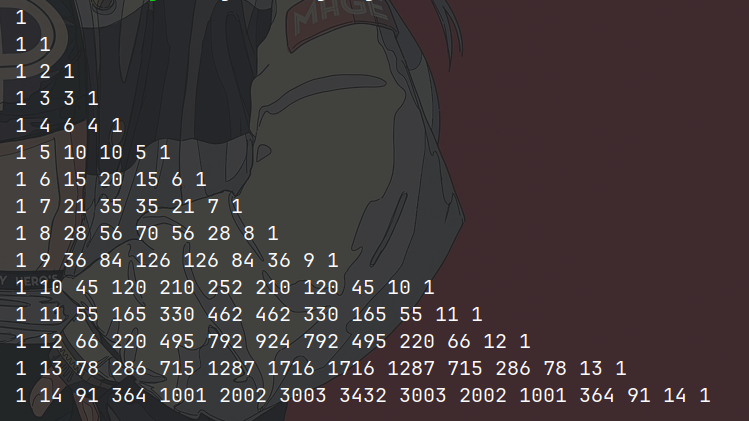
\includegraphics[width=.9\textwidth]{\reportDirectory/demo.png}
    \caption{Трикутник паскаля для $n = 15$}
    \label{fig:task}
\end{figure}


\newpage
\subsection{Порівняння усіх алгоритмів}
\begin{figure}[h!]
    \centering
    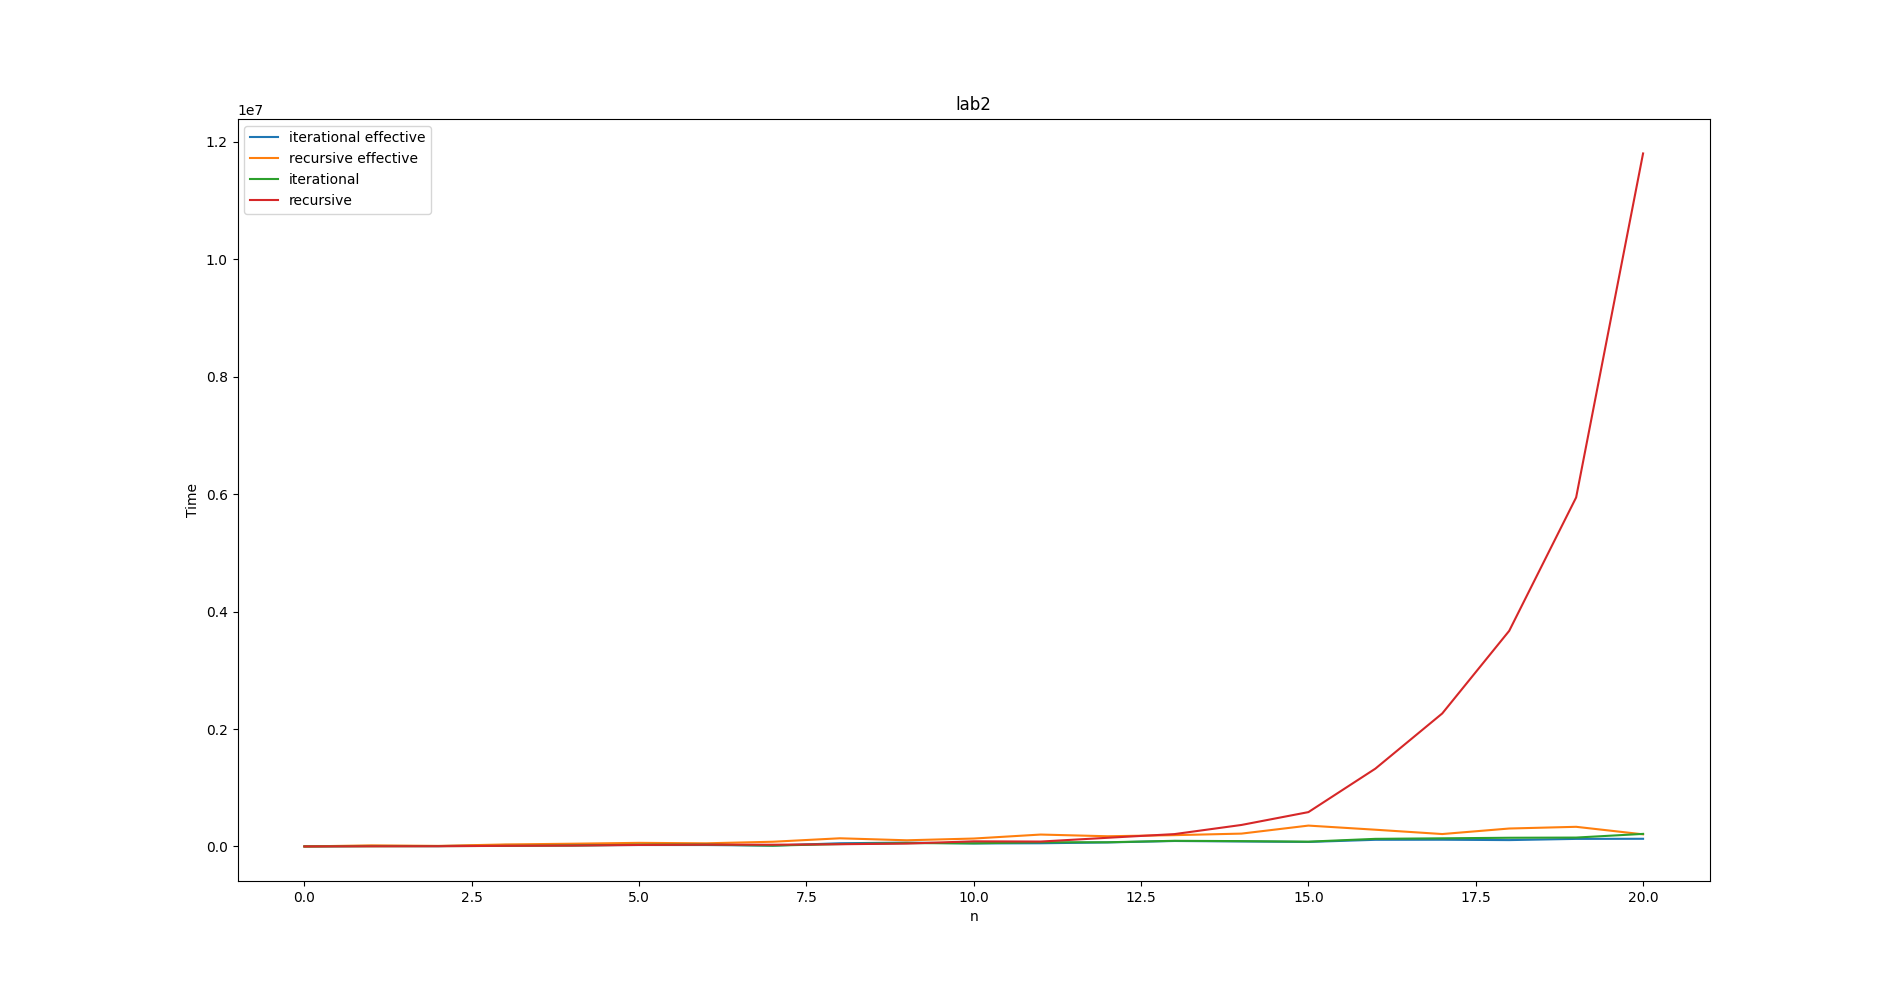
\includegraphics[width=\textwidth]{\reportDirectory/compare1.png}
    \caption{Порівняння усіх алгоритмів при $n = 20$}
    \label{fig:task}
\end{figure}

\begin{figure}[h!]
    \centering
    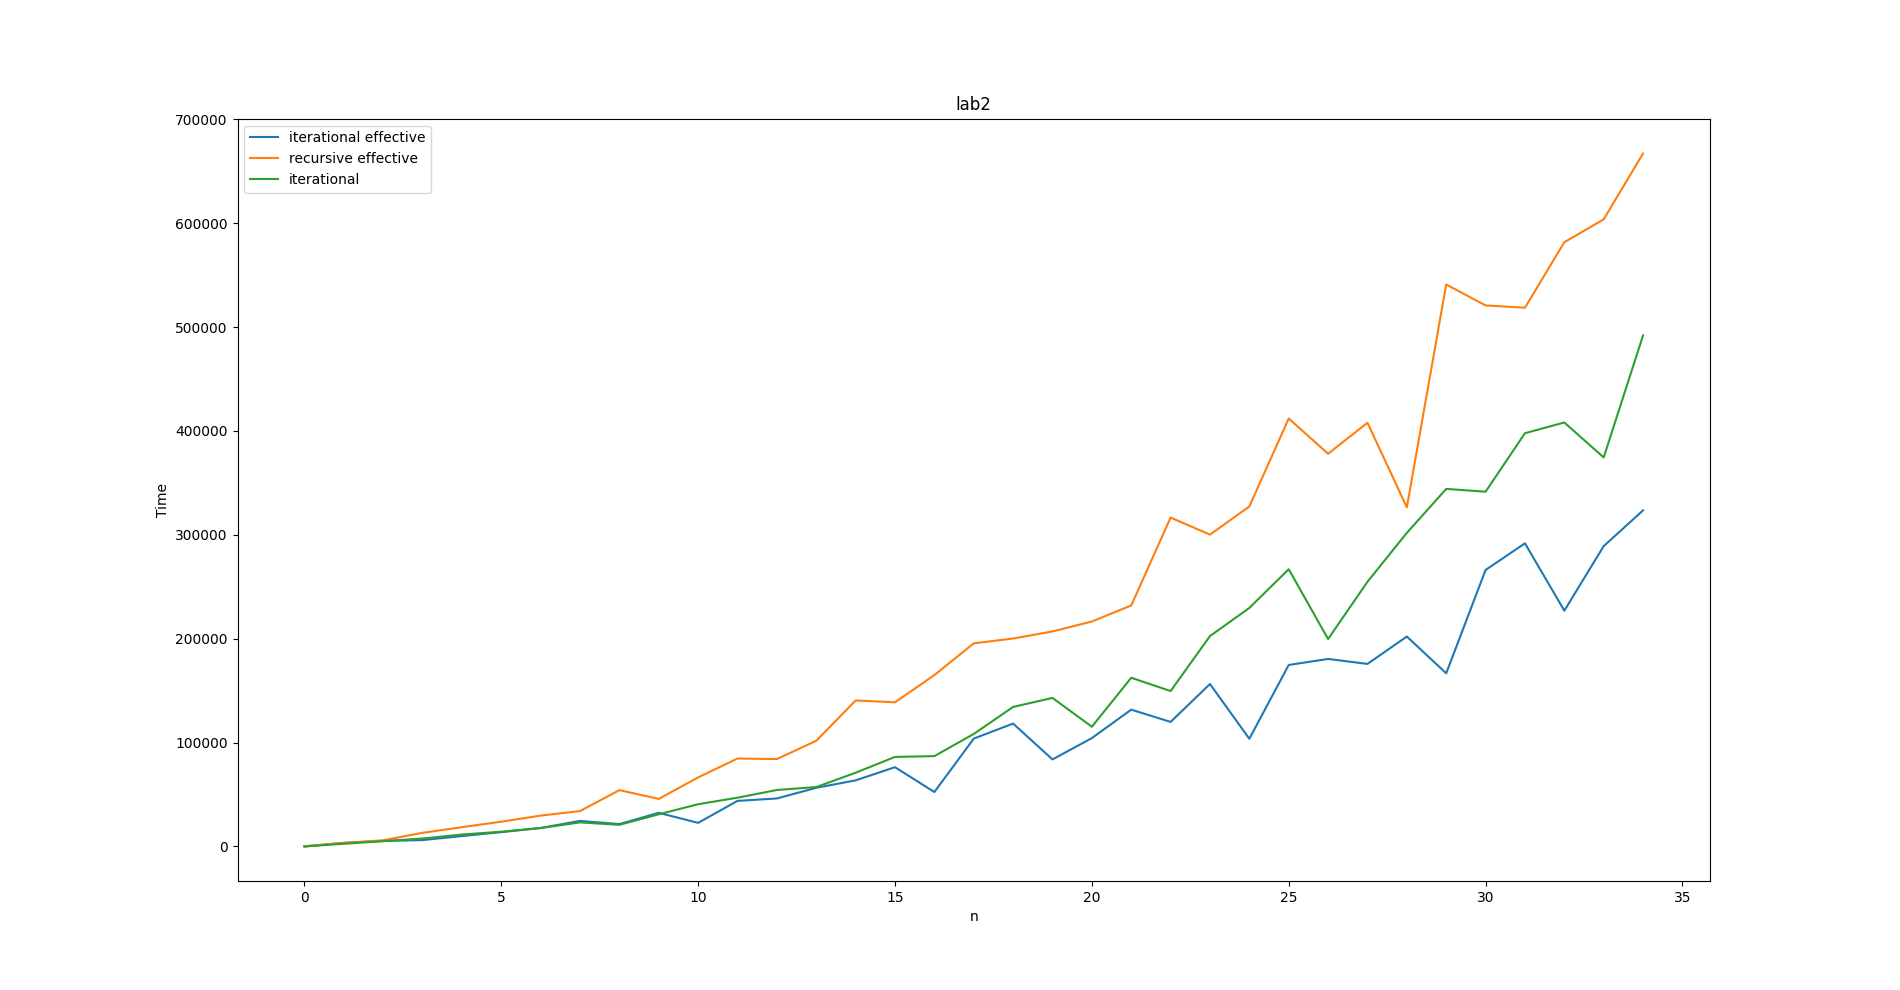
\includegraphics[width=\textwidth]{\reportDirectory/compare2.png}
    \caption{Порівняння усіх алгоритмів окрім не ефективного рекурсивного при\\$n = 34$}
    \label{fig:task}
\end{figure}


\newpage
\section{Висновки}
В ході виконання лабораторної робити було порівняно складність роботи ітераційного та рекурсивного варіанту алгоримту,
а також знайдено найоптимальніший алгоритм з розібраних, їм виявився ефективний варіант ітераційного алгоритму,
проте він потребує $O(n)$ додаткового місця. Тому якщо потрібно $O(1)$ місця,
то буде краще скористатися наівною реалізацією ітераційного алгоритму. 
